\documentclass[12pt, twoside]{book}
%\documentclass[12pt, oneside]{book}  % jednostranna tlac
\usepackage[a4paper,top=2.5cm,bottom=2.5cm,left=3.5cm,right=2cm]{geometry}
\usepackage[utf8]{inputenc}
\usepackage[T1]{fontenc}
\usepackage{graphicx}
\usepackage{url}
\usepackage[hidelinks,breaklinks]{hyperref}
\usepackage[table,xcdraw]{xcolor} % Added for table coloring
\usepackage[semicolon,round,sort&compress,sectionbib]{natbib}
\usepackage{multirow} % Multirow tables
\usepackage{listings} % Code
\usepackage{algorithm2e} % Pseudocode
%\usepackage[slovak]{babel} % vypnite pre prace v anglictine
\linespread{1.25} % hodnota 1.25 by mala zodpovedat 1.5 riadkovaniu

\usepackage{amsmath}
\usepackage{amssymb}

% pridane cary
% \def\lg{\mathop{\mathrm{lg}}}  \lg
\newtheorem{theorem}{Theorem} % https://www.overleaf.com/learn/latex/theorems_and_proofs
\newtheorem{definition}{Definition}
\def\ceil#1{\left\lceil #1 \right\rceil}
\def\floor#1{\left\lfloor #1 \right\rfloor}
\def\access{\mathit{access}}
\def\rank{\mathit{rank}}
\def\select{\mathit{select}}
\def\countOp{\mathit{count}}
\def\extractOp{\mathit{extract}}
\def\locateOp{\mathit{locate}}
\def\BigO{\mathcal{O}}
\def\Count{\mathit{Count}}
\def\Lex{\mathit{Lex}}
\def\prec{<}

\RestyleAlgo{ruled}

% Listings
\lstset{
  aboveskip=1ex,
  backgroundcolor=\color{gray!10},
  basicstyle=\small\ttfamily,
  belowskip=1ex,
  breaklines=true,
  columns=fullflexible,
  framerule=0pt,
  framexrightmargin=0em,
  framexleftmargin=0em,
  numbers=left,
  numberstyle=\footnotesize\sffamily,
  tabsize=2
}

% -------------------
% --- Definicia zakladnych pojmov
% --- Vyplnte podla vasho zadania
% -------------------
\def\mfrok{2022}
\def\mfnazov{Engineering compressed bit vectors}
\def\mftyp{Master's Thesis}
\def\mfautor{Bc. Andrej Korman}
\def\mfskolitel{Mgr. Jakub Kováč, PhD.}

%ak mate konzultanta, odkomentujte aj jeho meno na titulnom liste
%\def\mfkonzultant{doc. Mgr. Bronislava Brejová, PhD.}  

\def\mfmiesto{Bratislava, \mfrok}

% bioinformatici odkomentujú riadok s dvoma odbormi a iný program
\def\mfodbor{Computer Science}
\def\program{Computer Science}

% Ak je školiteľ z FMFI, uvádzate katedru školiteľa, zrejme by mala byť aj na zadaní z AIS2
% Ak máte externého školiteľa, uvádzajte Katedru informatiky
\def\mfpracovisko{Department of Computer Science}

\begin{document}     
\frontmatter


% -------------------
% --- Obalka ------
% -------------------
\thispagestyle{empty}

\begin{center}
  \sc\large
  Comenius University in Bratislava\\
  Faculty of Mathematics, Physics and Informatics

\vfill

{\LARGE\mfnazov}\\
\mftyp
\end{center}

\vfill

{\sc\large 
\noindent \mfrok\\
\mfautor
}

\cleardoublepage
% --- koniec obalky ----

% -------------------
% --- Titulný list
% -------------------

\thispagestyle{empty}
\noindent

\begin{center}
\sc  
\large
  Comenius University in Bratislava\\
  Faculty of Mathematics, Physics and Informatics

\vfill

{\LARGE\mfnazov}\\
\mftyp
\end{center}

\vfill

\noindent
\begin{tabular}{ll}
Study Programme: & \program \\
Field of Study: & \mfodbor \\
Department: & \mfpracovisko \\
Supervisor: & \mfskolitel \\
% Consultant: & \mfkonzultant \\
\end{tabular}

\vfill


\noindent \mfmiesto\\
\mfautor

\cleardoublepage
% --- Koniec titulnej strany


% -------------------
% --- Zadanie z AIS
% -------------------
% v tlačenej verzii s podpismi zainteresovaných osôb.
% v elektronickej verzii sa zverejňuje zadanie bez podpisov
% v pracach v aglictine anglicke aj slovenske zadanie

\newpage 
\thispagestyle{empty}
\hspace{-2cm}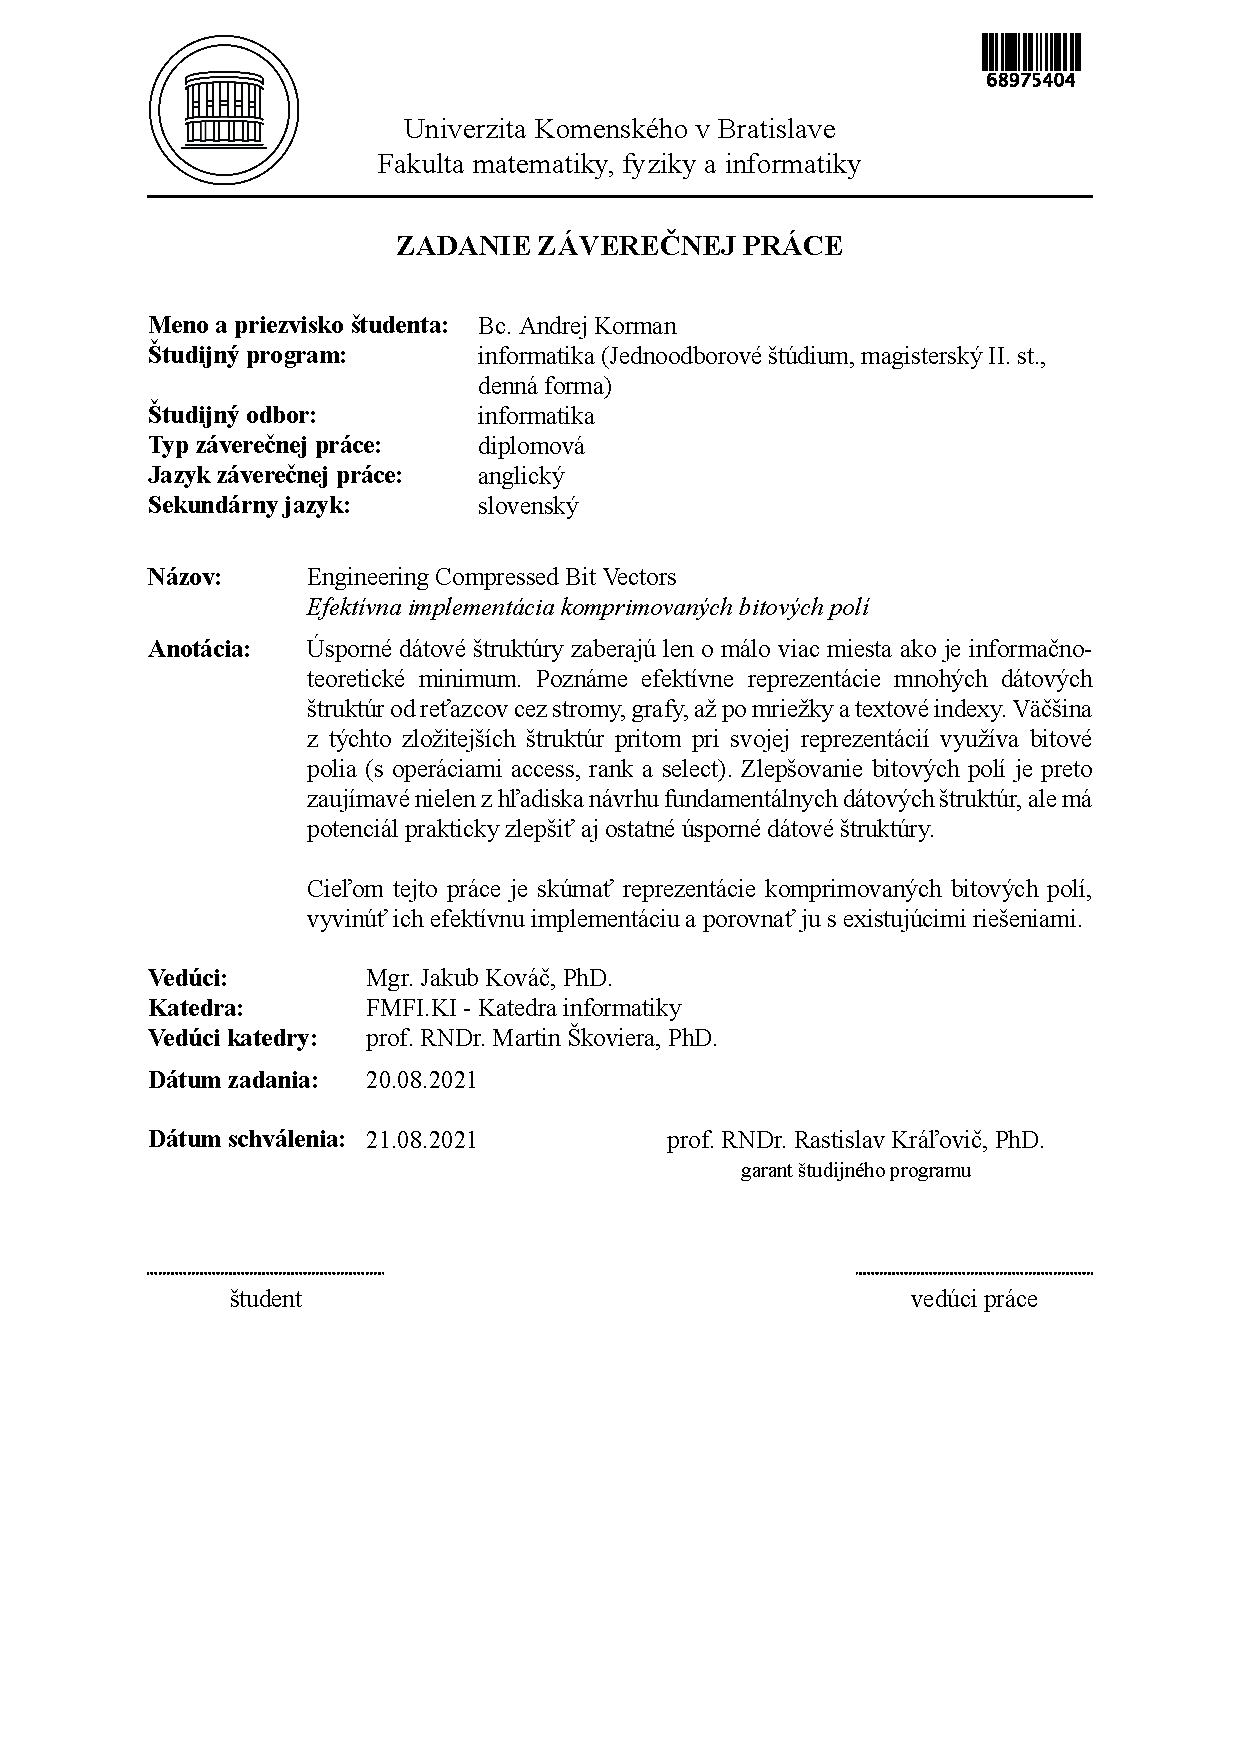
\includegraphics[width=1.1\textwidth]{images/zadanie}

\hspace{-2cm}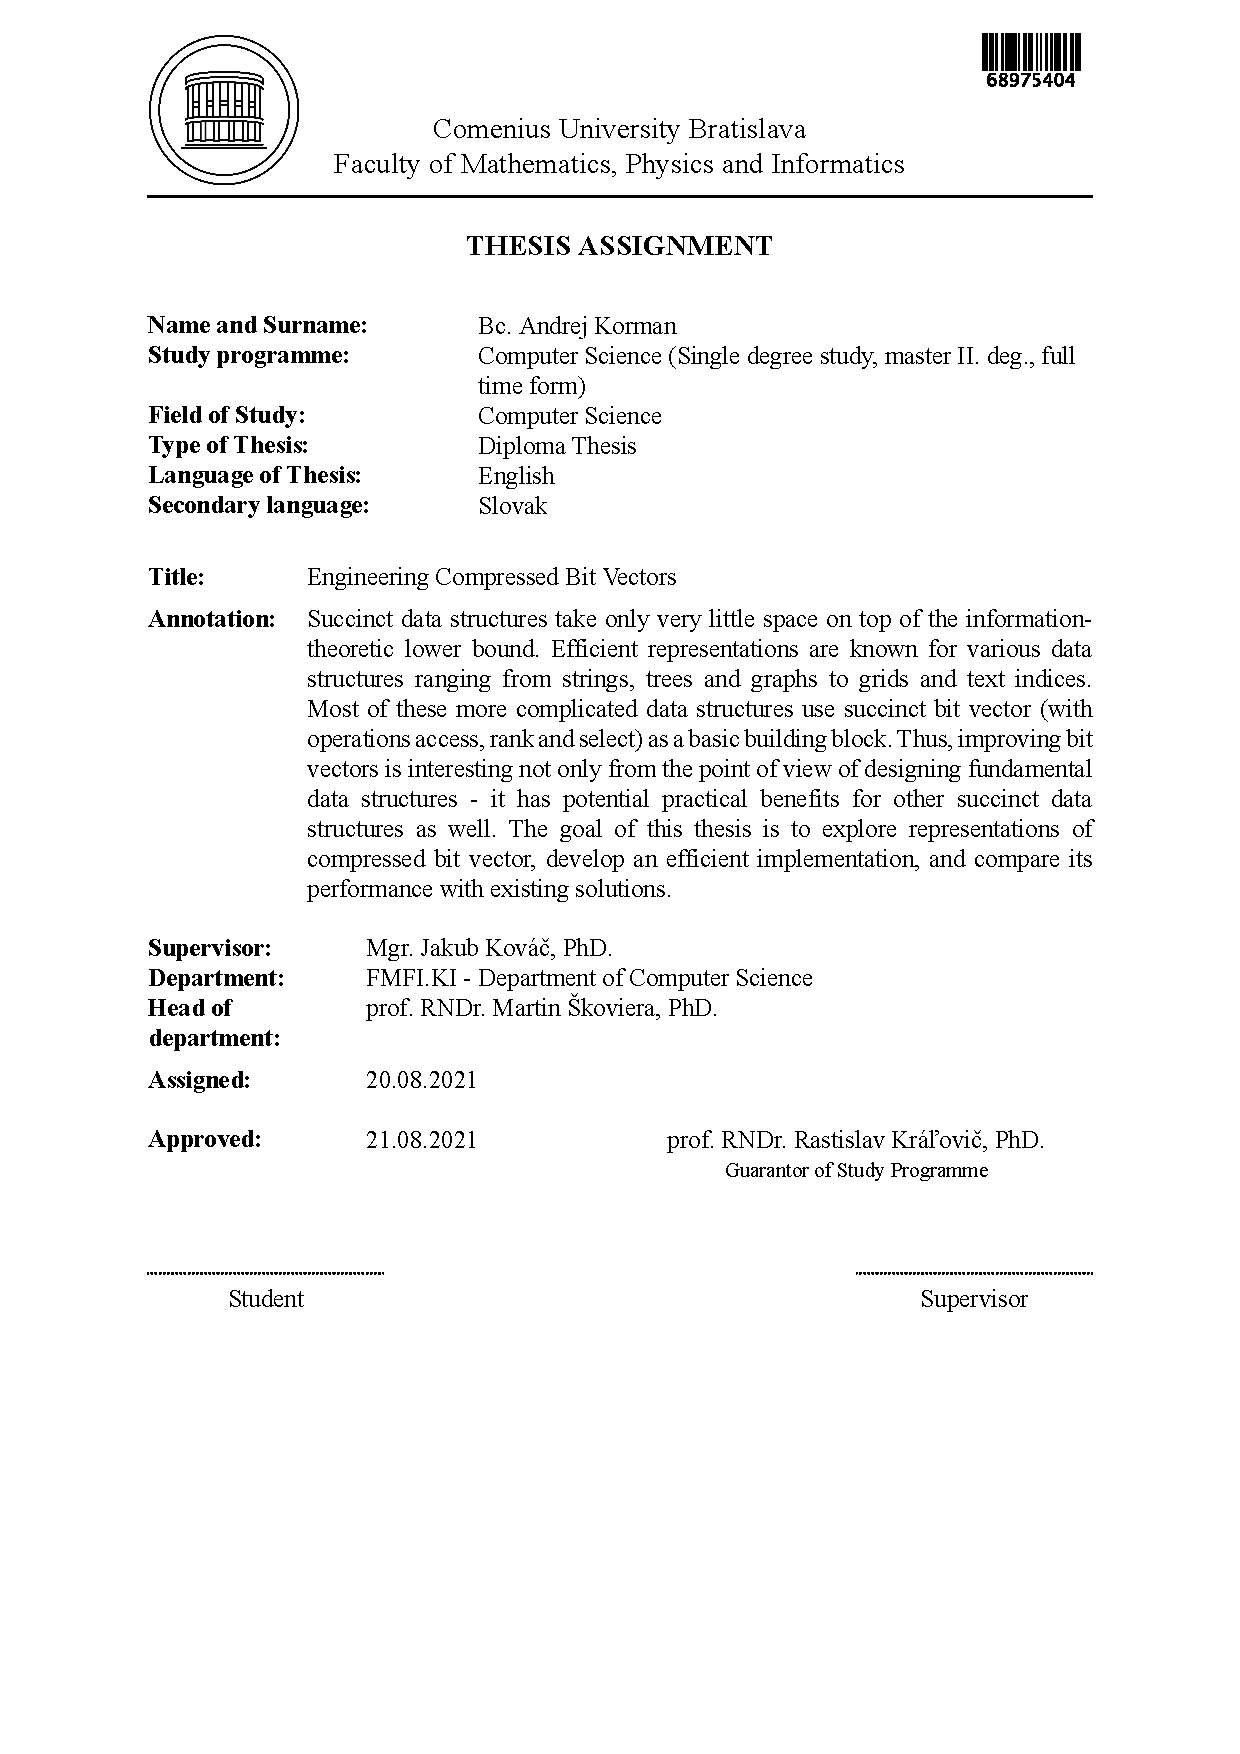
\includegraphics[width=1.1\textwidth]{images/zadanie-en}

% --- Koniec zadania

\frontmatter

% -------------------
%   Poďakovanie - nepovinné
% -------------------
\setcounter{page}{3}
\newpage 
~

\vfill
{\bf Acknowledgments:} Tu môžete poďakovať školiteľovi, prípadne
ďalším osobám, ktoré vám s prácou nejako pomohli, poradili,
poskytli dáta a podobne.

% --- Koniec poďakovania

% -------------------
%   Abstrakt - Slovensky
% -------------------
\newpage 
\section*{Abstrakt}

Úsporné dátove štruktúry sú užitočnými v prípadoch keď pracujeme s veľkým
objemom dát a klasické dátové štruktúry nás limitujú
svojími pamäťovými nárokmi. Bitové pole s operáciami $\access$,
$\rank$ a $\select$ je stavebným kameňom mnohých prakticky užitočných
úsporných dátových štruktúr. V našej práci sa venujeme implementácii
bitového poľa pomocou metódy \textit{RRR}, ktorá delí postupnosť bitov na
bloky, ktoré sú ďalej jednotlivo komprimované. V tejto práci sme
predstavili nový spôsob kompresie a dekompresie blokov pre všeobecné
bitové polia ale aj novú metódu, ktorá výmenou za nekódovanie niektorých
blokov šetrí priestor na reprezentácii ostatných. Obidve tieto
myšlienky sme naimplementovali a experimentálne otestovali v umelých
ale aj reálnych podmienkach ako je napr. FM-index, ktorý rieši problém
vyhľadávanie vzorky v texte.

\paragraph*{Kľúčové slová:} bitové pole, úsporné dátové štruktúry
% --- Koniec Abstrakt - Slovensky


% -------------------
% --- Abstrakt - Anglicky 
% -------------------
\newpage 
\section*{Abstract}

Abstract in the English language (translation of the abstract in the
Slovak language).


\paragraph*{Keywords:} bit vector, succinct data structures

% --- Koniec Abstrakt - Anglicky

% -------------------
% --- Predhovor - v informatike sa zvacsa nepouziva
% -------------------
%\newpage 
%\thispagestyle{empty}
%
%\huge{Predhovor}
%\normalsize
%\newline
%Predhovor je všeobecná informácia o práci, obsahuje hlavnú charakteristiku práce 
%a okolnosti jej vzniku. Autor zdôvodní výber témy, stručne informuje o cieľoch 
%a význame práce, spomenie domáci a zahraničný kontext, komu je práca určená, 
%použité metódy, stav poznania; autor stručne charakterizuje svoj prístup a svoje 
%hľadisko. 
%
% --- Koniec Predhovor


% -------------------
% --- Obsah
% -------------------

\newpage 

\tableofcontents

% ---  Koniec Obsahu

% -------------------
% --- Zoznamy tabuliek, obrázkov - nepovinne
% -------------------

\newpage 

% \listoffigures
% \listoftables

% ---  Koniec Zoznamov

\mainmatter


%\input uvod.tex 

\input kapitola1.tex

\input kapitola2.tex

\input kapitola3.tex

\input kapitola4.tex

%\input kapitola5.tex

%\input latex.tex

%\input lorem.tex

\input zaver.tex

% -------------------
% --- Bibliografia
% -------------------


\newpage	

\backmatter

\thispagestyle{empty}
\clearpage

\bibliographystyle{chicago}
\bibliography{literatura} 

%Prípadne môžete napísať literatúru priamo tu
%\begin{thebibliography}{5}
 
%\bibitem{br1} MOLINA H. G. - ULLMAN J. D. - WIDOM J., 2002, Database Systems, Upper Saddle River : Prentice-Hall, 2002, 1119 s., Pearson International edition, 0-13-098043-9

%\bibitem{br2} MOLINA H. G. - ULLMAN J. D. - WIDOM J., 2000 , Databasse System implementation, New Jersey : Prentice-Hall, 2000, 653s., ???

%\bibitem{br3} ULLMAN J. D. - WIDOM J., 1997, A First Course in Database Systems, New Jersey : Prentice-Hall, 1997, 470s., 

%\bibitem{br4} PREFUSE, 2007, The Prefuse visualization toolkit,  [online] Dostupné na internete: <http://prefuse.org/>

%\bibitem{br5} PREFUSE Forum, Sourceforge - Prefuse Forum,  [online] Dostupné na internete: <http://sourceforge.net/projects/prefuse/>

%\end{thebibliography}

%---koniec Referencii

% -------------------
%--- Prilohy---
% -------------------

%Nepovinná časť prílohy obsahuje materiály, ktoré neboli zaradené priamo  do textu. Každá príloha sa začína na novej strane.
%Zoznam príloh je súčasťou obsahu.
%
\input appendixA.tex

%\input appendixB.tex

\end{document}